\subsection{Caso de estudio 2}

Para este segundo caso de estudio, se tendrán en cuenta los accidentes comprendidos desde las 12 horas a las 6 horas(a.m para un caso y p.m para el opuesto) en Andalucía, para ver como difieren las cifras de víctimas comparando por el día y por la madrugada.

\subsubsection{Primera franja horaria: 12-6 a.m}

\begin{figure}[H]
\begin{subfigure}{.5\textwidth}
  \centering
  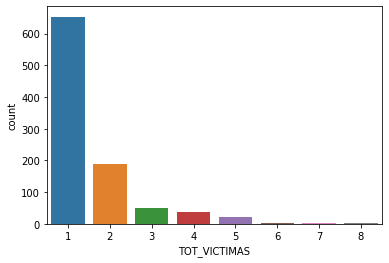
\includegraphics[width=0.8\textwidth]{imagenes/victimas_caso2.png}
  \caption{Número de victimas de 12 a 6 a.m}
  \label{fig:sfig1}
\end{subfigure}%
\begin{subfigure}{.5\textwidth}
  \centering
  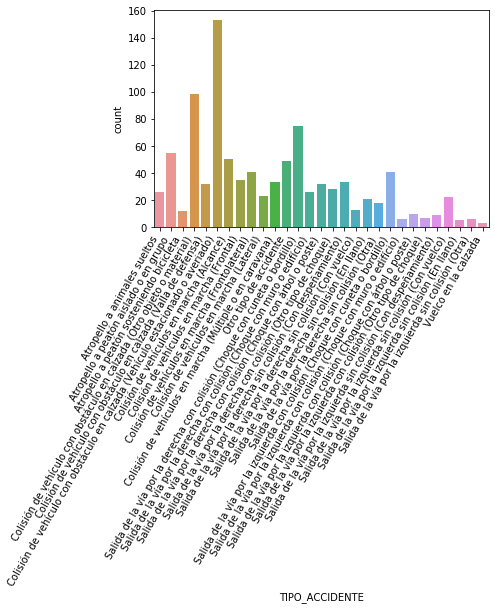
\includegraphics[width=0.8\textwidth]{imagenes/tipo_accidente_caso2.png}
  \caption{Tipo de accidentes en intersecciones de 12 a 6 a.m}
  \label{fig:sfig2}
\end{subfigure}
\caption{Víctimas y tipos de accidente en intersecciones de 12 a 6 a.m}
\label{fig:fig}
\end{figure}

\paragraph{Resultados de la segmentación}

\begin{table}[H]
%1
\begin{subtable}[H]{0.45\textwidth}
        \centering
\begin{tabular}{|c|c|c|}
\hline
\textit{k = 3}      & \textbf{K-Means}           & \textbf{Agg-Clustering} \\ \hline
\textbf{Silhouette} & \textit{\textbf{0,5659}}   & \textit{0,5519}         \\ \hline
\textbf{Calinsky}   & \textit{\textbf{573,8087}} & 479,1132                \\ \hline
\end{tabular}
\end{subtable}
\hfill
\begin{subtable}[H]{0.45\textwidth}
        \centering
\begin{tabular}{|c|c|c|}
\hline
\textit{k = 4}      & \textbf{K-Means}           & \textbf{Agg-Clustering} \\ \hline
\textbf{Silhouette} & \textit{\textbf{0,5813}}   & \textit{0,5736}         \\ \hline
\textbf{Calinsky}   & \textit{\textbf{582,3789}} & 495,6096                \\ \hline
\end{tabular}
\end{subtable}
%2
\begin{subtable}[H]{0.45\textwidth}
        \centering
\begin{tabular}{|c|c|c|}
\hline
\textit{k = 5}      & \textbf{K-Means}           & \textbf{Agg-Clustering} \\ \hline
\textbf{Silhouette} & \textit{\textbf{0,6309}}   & \textit{0,5629}         \\ \hline
\textbf{Calinsky}   & \textit{\textbf{659,8113}} & 555,6438                \\ \hline
\end{tabular}
\end{subtable}
\hfill
\begin{subtable}[H]{0.45\textwidth}
        \centering
\begin{tabular}{|c|c|c|}
\hline
\textit{k = 6}      & \textbf{K-Means}           & \textbf{Agg-Clustering}  \\ \hline
\textbf{Silhouette} & \textit{0,7001}            & \textit{\textbf{0,7026}} \\ \hline
\textbf{Calinsky}   & \textit{\textbf{685,6643}} & 657,3857                 \\ \hline
\end{tabular}
\end{subtable}
%3
\begin{subtable}[H]{0.45\textwidth}
        \centering
\begin{tabular}{|c|c|c|}
\hline
\textit{k = 7}      & \textbf{K-Means}  & \textbf{Agg-Clustering}    \\ \hline
\textbf{Silhouette} & \textit{0,6734}   & \textit{\textbf{0,7088}}   \\ \hline
\textbf{Calinsky}   & \textit{629,0390} & \textit{\textbf{643,1446}} \\ \hline
\end{tabular}
\end{subtable}
\hfill
\caption{Resultados obtenidos con los distintos algoritmos para el tramo de la madrugada(12-6 a.m)}
\end{table}

Ocurre algo parecido en parte al primer caso de estudio, el valor de Silhouette es parecido para ambos algoritmos excepto en algunos casos($k=5$ y $k=7$). Con el índice Calinski podemos ver que para $k=6$ usando K-Means obtiene el mejor resultado entre los valores de $k$ escogidos, por lo que podríamos decir que es el mejor agrupado. Aun empatando con Agg para $k=7$ tiene mejor Calinski.

\paragraph{Interpretación de la segmentación}

\begin{figure}[H]
\begin{subfigure}{.5\textwidth}
  \centering
  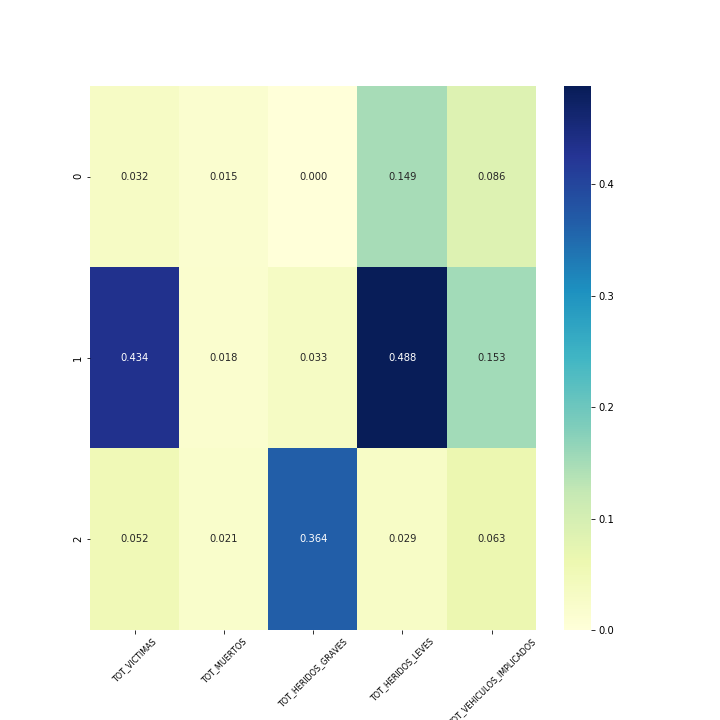
\includegraphics[width=0.9\textwidth]{imagenes/case2/kmeans/heatmaps/hm_kmeans_case2_salida_k3.png}
\end{subfigure}%
\begin{subfigure}{.5\textwidth}
  \centering
  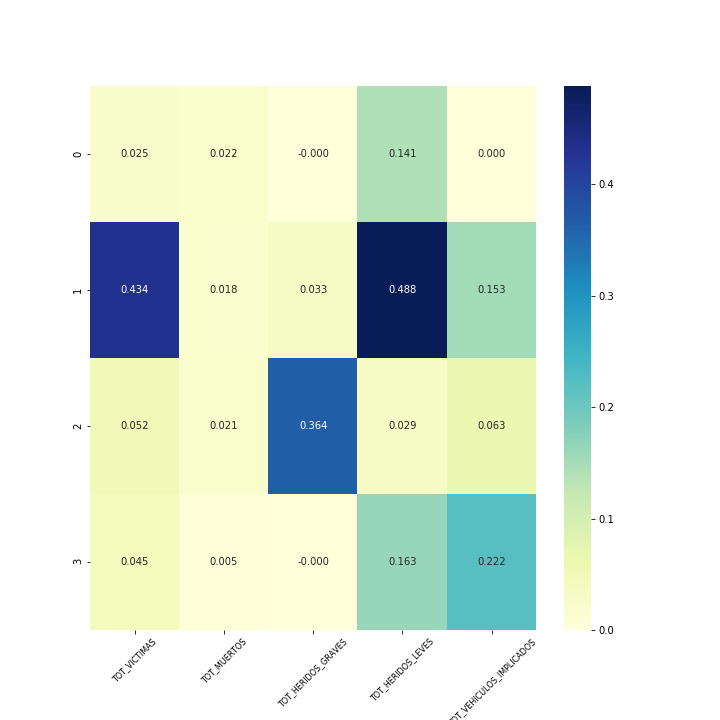
\includegraphics[width=0.9\textwidth]{imagenes/case2/kmeans/heatmaps/hm_kmeans_case2_salida_k4.png}
\end{subfigure}
\begin{subfigure}{.5\textwidth}
  \centering
  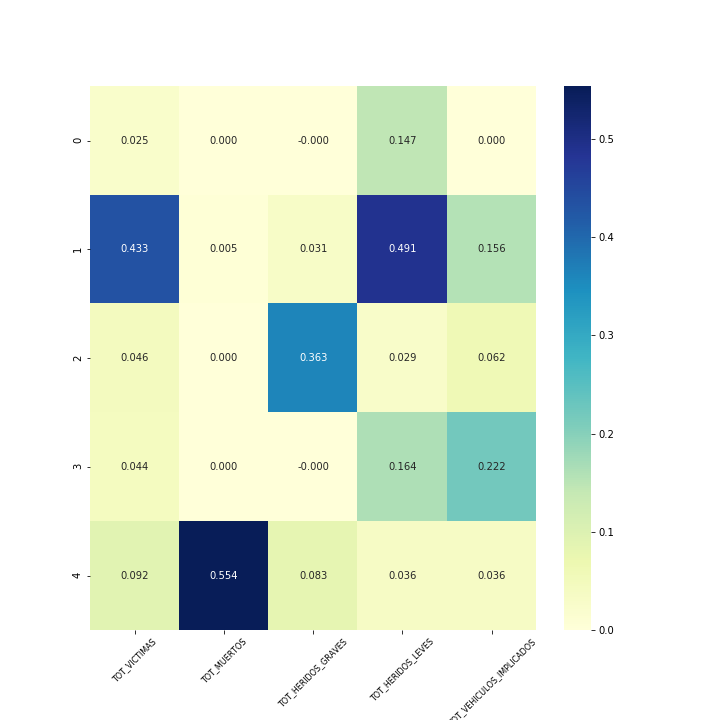
\includegraphics[width=0.9\textwidth]{imagenes/case2/kmeans/heatmaps/hm_kmeans_case2_salida_k5.png}
\end{subfigure}
\begin{subfigure}{.5\textwidth}
  \centering
  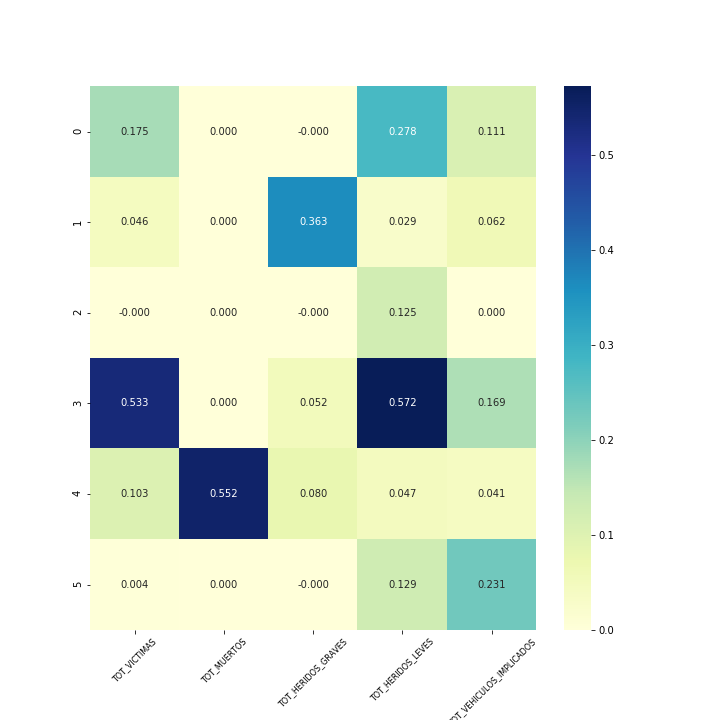
\includegraphics[width=0.9\textwidth]{imagenes/case2/kmeans/heatmaps/hm_kmeans_case2_salida_k6.png}
\end{subfigure}
\begin{subfigure}{.5\textwidth}
  \centering
  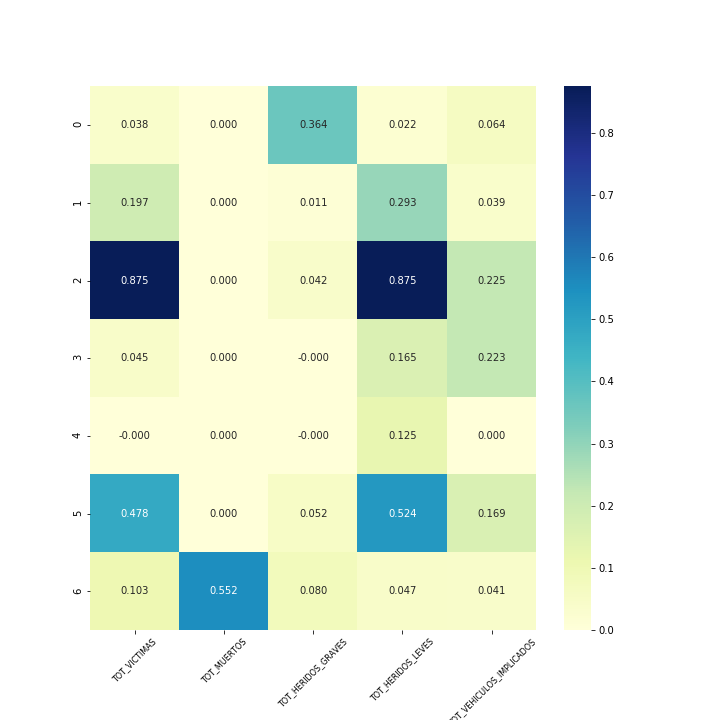
\includegraphics[width=0.9\textwidth]{imagenes/case2/kmeans/heatmaps/hm_kmeans_case2_salida_k7.png}
\end{subfigure}
\caption{Mapas de calor para el algoritmo K-Means, A.M}
\label{fig:hm-km}
\end{figure}

\begin{figure}[H]
\begin{subfigure}{.5\textwidth}
  \centering
  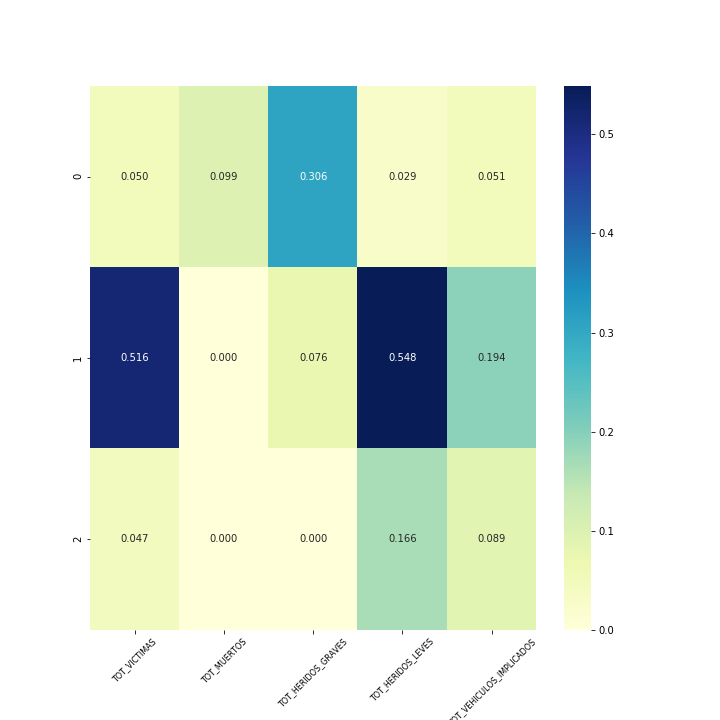
\includegraphics[width=0.9\textwidth]{imagenes/case2/agglomerative/heatmaps/hm_agglomerative_case2_salida_k3.png}
\end{subfigure}%
\begin{subfigure}{.5\textwidth}
  \centering
  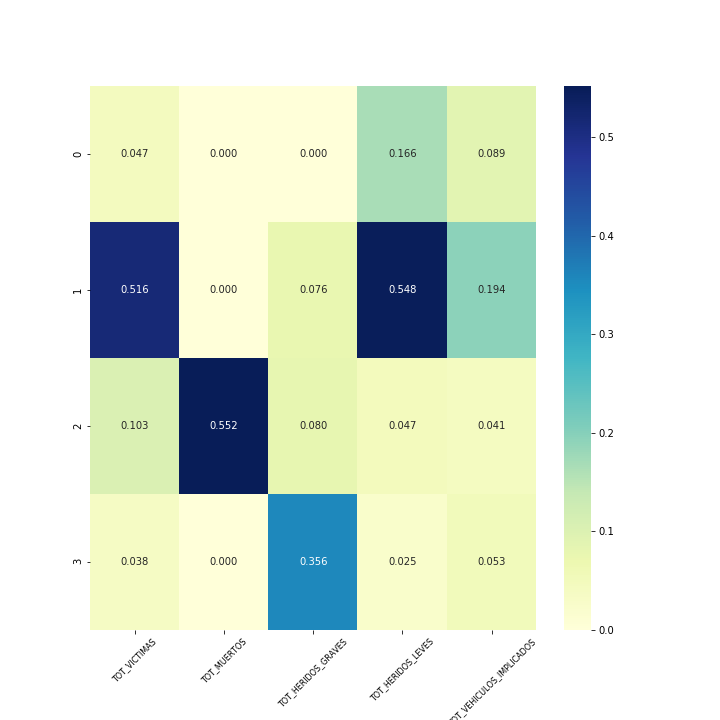
\includegraphics[width=0.9\textwidth]{imagenes/case2/agglomerative/heatmaps/hm_agglomerative_case2_salida_k4.png}
\end{subfigure}
\begin{subfigure}{.5\textwidth}
  \centering
  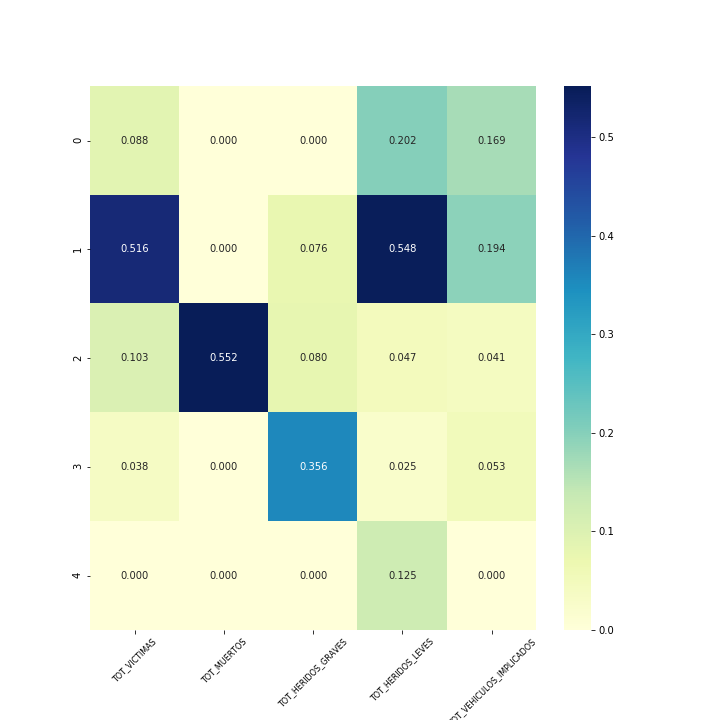
\includegraphics[width=0.9\textwidth]{imagenes/case2/agglomerative/heatmaps/hm_agglomerative_case2_salida_k5.png}
\end{subfigure}
\begin{subfigure}{.5\textwidth}
  \centering
  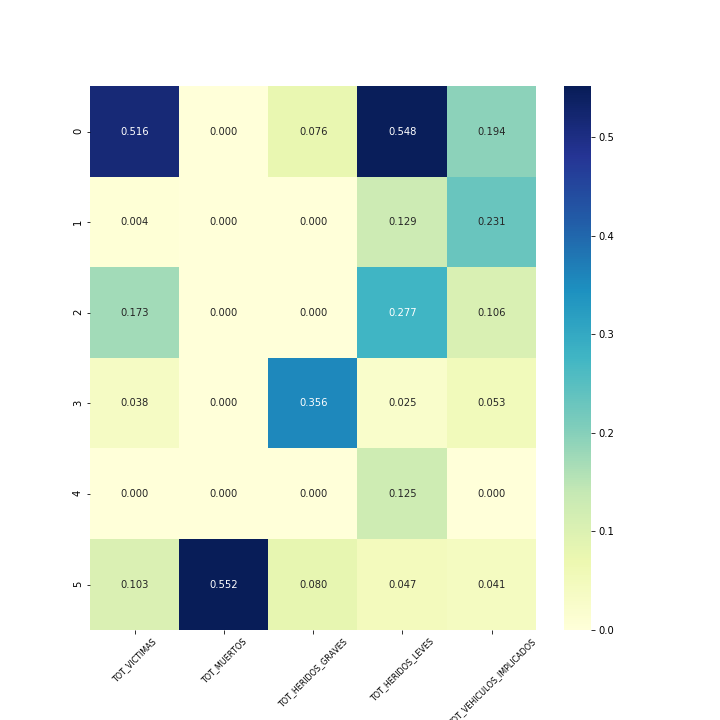
\includegraphics[width=0.9\textwidth]{imagenes/case2/agglomerative/heatmaps/hm_agglomerative_case2_salida_k6.png}
\end{subfigure}
\begin{subfigure}{.5\textwidth}
  \centering
  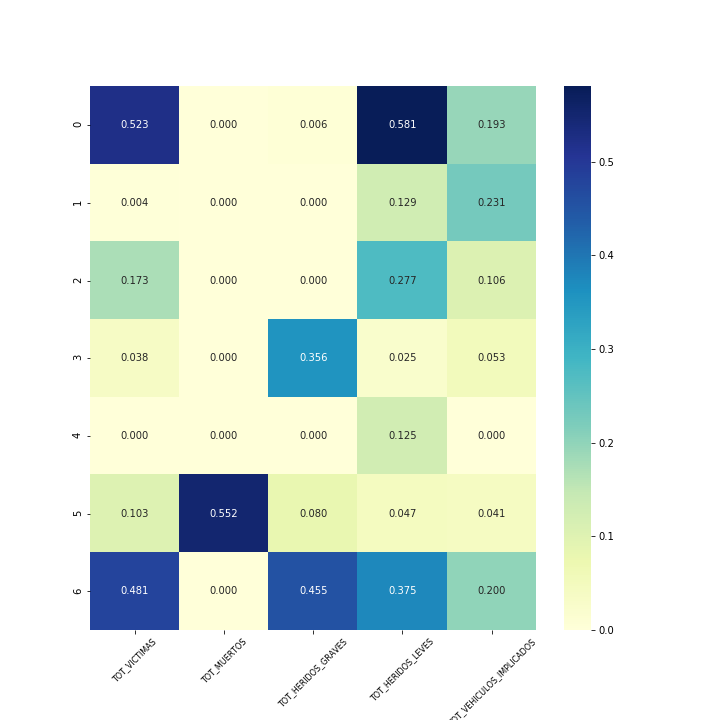
\includegraphics[width=0.9\textwidth]{imagenes/case2/agglomerative/heatmaps/hm_agglomerative_case2_salida_k7.png}
\end{subfigure}
\caption{Mapas de calor para el algoritmo Agglomerative Clustering, A.M}
\label{fig:hm-km}
\end{figure}

\begin{figure}[H]
\begin{subfigure}{.5\textwidth}
  \centering
  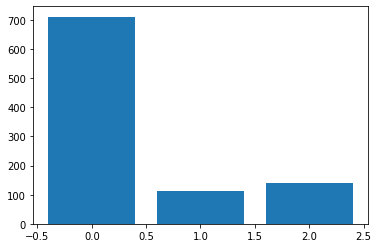
\includegraphics[width=0.45\textwidth]{imagenes/counter/am/km3.png}
  \caption{$k=3$}
\end{subfigure}%
\begin{subfigure}{.5\textwidth}
  \centering
  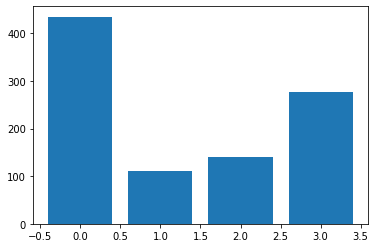
\includegraphics[width=0.45\textwidth]{imagenes/counter/am/km4.png}
  \caption{$k=4$}
\end{subfigure}
\begin{subfigure}{.5\textwidth}
  \centering
  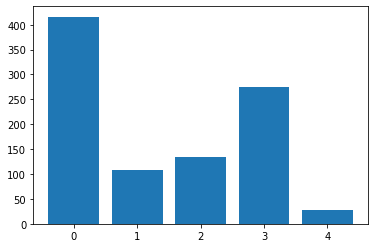
\includegraphics[width=0.45\textwidth]{imagenes/counter/am/km5.png}
  \caption{$k=5$}
\end{subfigure}
\begin{subfigure}{.5\textwidth}
  \centering
  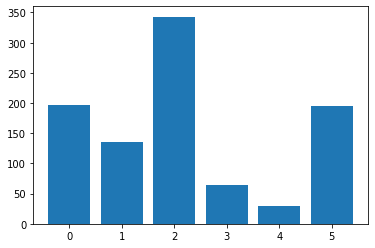
\includegraphics[width=0.45\textwidth]{imagenes/counter/am/km6.png}
  \caption{$k=6$}
\end{subfigure}
\begin{subfigure}{.5\textwidth}
  \centering
  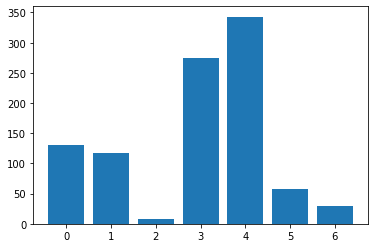
\includegraphics[width=0.45\textwidth]{imagenes/counter/am/km7.png}
  \caption{$k=7$}
\end{subfigure}
\caption{Número de instancias en cada cluster(K-Means), A.M}
\label{fig:hm-km}
\end{figure}


\begin{figure}[H]
\begin{subfigure}{.5\textwidth}
  \centering
  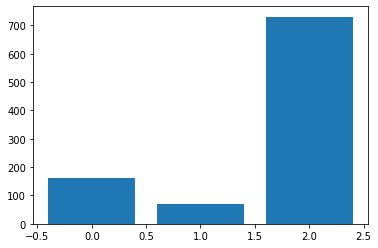
\includegraphics[width=0.45\textwidth]{imagenes/counter/am/agg3.png}
  \caption{$k=3$}
\end{subfigure}%
\begin{subfigure}{.5\textwidth}
  \centering
  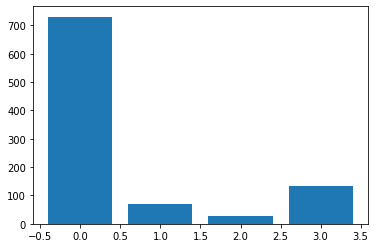
\includegraphics[width=0.45\textwidth]{imagenes/counter/am/agg4.png}
  \caption{$k=4$}
\end{subfigure}
\begin{subfigure}{.5\textwidth}
  \centering
  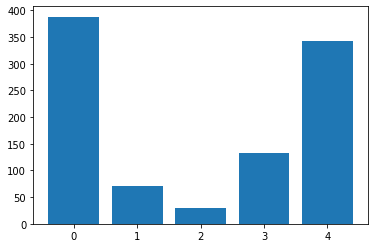
\includegraphics[width=0.45\textwidth]{imagenes/counter/am/agg5.png}
  \caption{$k=5$}
\end{subfigure}
\begin{subfigure}{.5\textwidth}
  \centering
  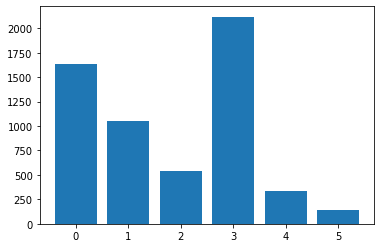
\includegraphics[width=0.45\textwidth]{imagenes/counter/am/agg6.png}
  \caption{$k=6$}
\end{subfigure}
\begin{subfigure}{.5\textwidth}
  \centering
  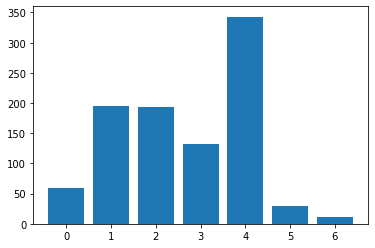
\includegraphics[width=0.45\textwidth]{imagenes/counter/am/agg7.png}
  \caption{$k=7$}
\end{subfigure}
\caption{Número de instancias en cada cluster(Agglomerative-Clustering), A.M}
\label{fig:hm-km}
\end{figure}


\subsubsection{Primera franja horaria: 12-6 p.m}

\begin{figure}[H]
\begin{subfigure}{.5\textwidth}
  \centering
  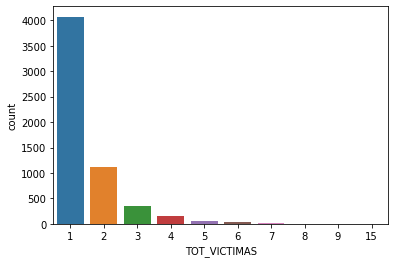
\includegraphics[width=0.8\textwidth]{imagenes/victimas_caso2-op.png}
  \caption{Número de victimas de 12 a 6 p.m}
  \label{fig:sfig1}
\end{subfigure}%
\begin{subfigure}{.5\textwidth}
  \centering
  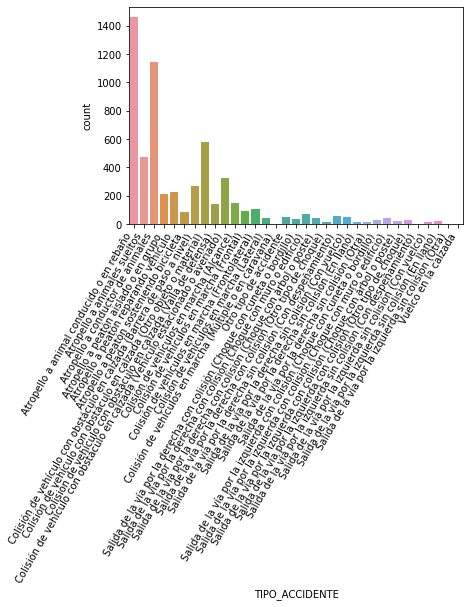
\includegraphics[width=0.8\textwidth]{imagenes/tipo_accidente_caso2-op.png}
  \caption{Tipo de accidentes en intersecciones de 12 a 6 p.m}
  \label{fig:sfig2}
\end{subfigure}
\caption{Víctimas y tipos de accidente en intersecciones de 12 a 6 p.m}
\label{fig:fig}
\end{figure}

Durante el día lo que predomina es el atropello ed animales conducidos o en rebaño y conductores de animales, seguido por animales sueltos y colisiones.

\paragraph{Resultados de la segmentación}

\begin{table}[H]
%1
\begin{subtable}[H]{0.45\textwidth}
        \centering
\begin{tabular}{|c|c|c|}
\hline
\textit{k = 3}      & \textbf{K-Means}             & \textbf{Agg-Clustering}  \\ \hline
\textbf{Silhouette} & \textit{0,5815}              & \textit{\textbf{0,5818}} \\ \hline
\textbf{Calinsky}   & \textit{\textbf{3.586,8308}} & \textit{3.533,2931}      \\ \hline
\end{tabular}
\end{subtable}
\hfill
\begin{subtable}[H]{0.45\textwidth}
        \centering
\begin{tabular}{|c|c|c|}
\hline
\textit{k = 4}      & \textbf{K-Means}             & \textbf{Agg-Clustering} \\ \hline
\textbf{Silhouette} & \textit{\textbf{0,6701}}     & \textit{0,6312}         \\ \hline
\textbf{Calinsky}   & \textit{\textbf{4.519,7336}} & \textit{3.758,7649}     \\ \hline
\end{tabular}
\end{subtable}
%2
\begin{subtable}[H]{0.45\textwidth}
        \centering
\begin{tabular}{|c|c|c|}
\hline
\textit{k = 5}      & \textbf{K-Means}             & \textbf{Agg-Clustering} \\ \hline
\textbf{Silhouette} & \textit{\textbf{0,6824}}     & \textit{0,6677}         \\ \hline
\textbf{Calinsky}   & \textit{\textbf{4.237,4522}} & \textit{3.785,2146}     \\ \hline
\end{tabular}
\end{subtable}
\hfill
\begin{subtable}[H]{0.45\textwidth}
        \centering
\begin{tabular}{|c|c|c|}
\hline
\textit{k = 6}      & \textbf{K-Means}             & \textbf{Agg-Clustering} \\ \hline
\textbf{Silhouette} & \textit{\textbf{0,7527}}     & \textit{0,7485}         \\ \hline
\textbf{Calinsky}   & \textit{\textbf{4.354,3507}} & \textit{4.127,1006}     \\ \hline
\end{tabular}
\end{subtable}
%3
\begin{subtable}[H]{0.45\textwidth}
        \centering
\begin{tabular}{|c|c|c|}
\hline
\textit{k = 7}      & \textbf{K-Means}             & \textbf{Agg-Clustering}  \\ \hline
\textbf{Silhouette} & \textit{0,7533}              & \textit{\textbf{0,7538}} \\ \hline
\textbf{Calinsky}   & \textit{\textbf{4.211,6426}} & \textit{4.077,9610}      \\ \hline
\end{tabular}
\end{subtable}
\hfill
\caption{Resultados obtenidos con los distintos algoritmos para el tramo del día(12-6 p.m)}
\end{table}

\paragraph{Interpretación de la segmentación}

\begin{figure}[H]
\begin{subfigure}{.5\textwidth}
  \centering
  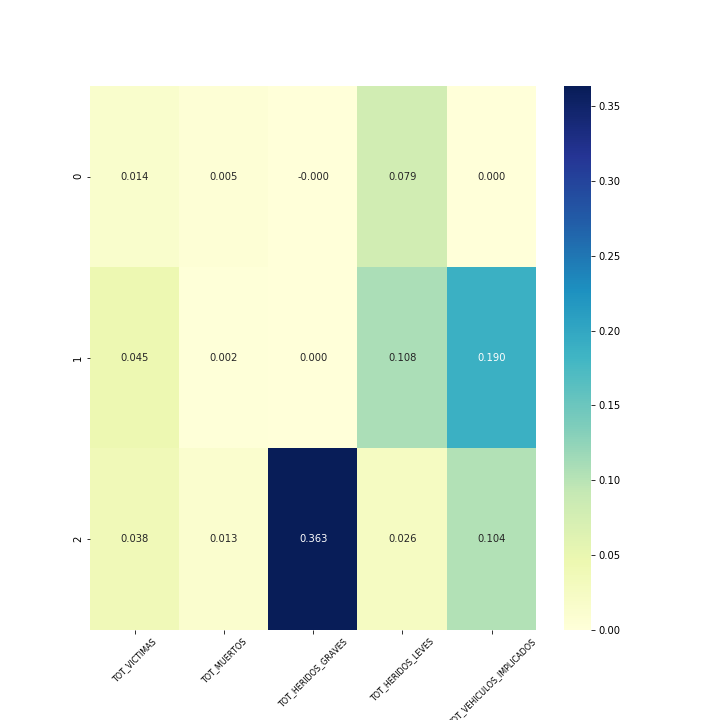
\includegraphics[width=0.9\textwidth]{imagenes/case2/kmeans/heatmaps/hm_kmeans_case2_entrada_k3.png}
\end{subfigure}%
\begin{subfigure}{.5\textwidth}
  \centering
  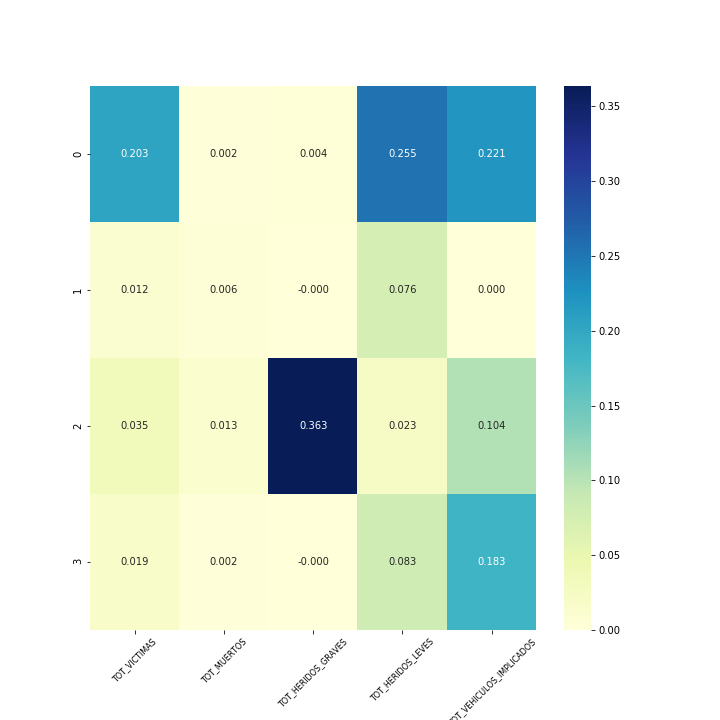
\includegraphics[width=0.9\textwidth]{imagenes/case2/kmeans/heatmaps/hm_kmeans_case2_entrada_k4.png}
\end{subfigure}
\begin{subfigure}{.5\textwidth}
  \centering
  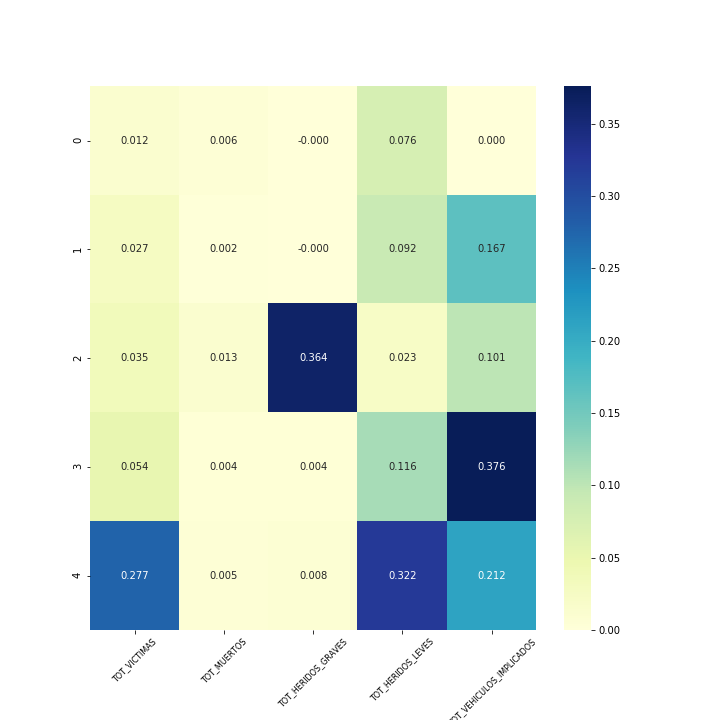
\includegraphics[width=0.9\textwidth]{imagenes/case2/kmeans/heatmaps/hm_kmeans_case2_entrada_k5.png}
\end{subfigure}
\begin{subfigure}{.5\textwidth}
  \centering
  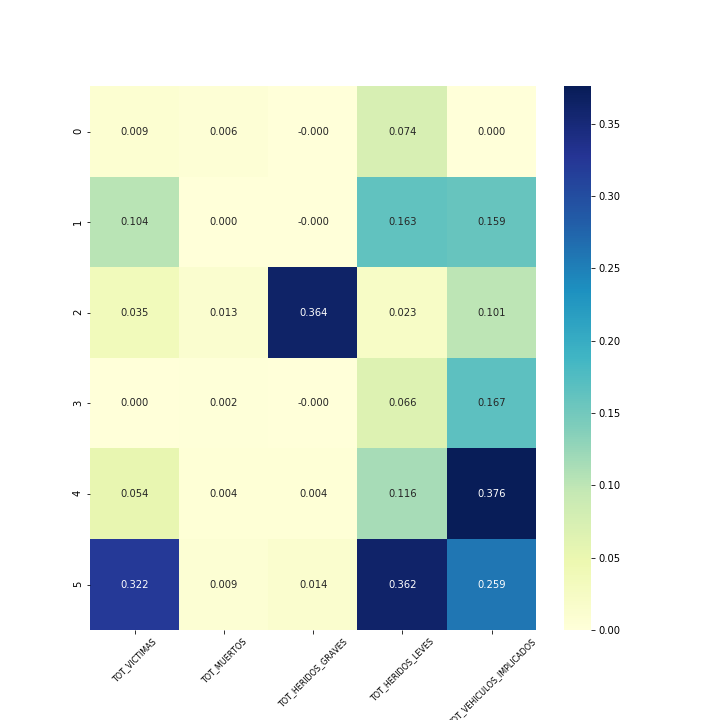
\includegraphics[width=0.9\textwidth]{imagenes/case2/kmeans/heatmaps/hm_kmeans_case2_entrada_k6.png}
\end{subfigure}
\begin{subfigure}{.5\textwidth}
  \centering
  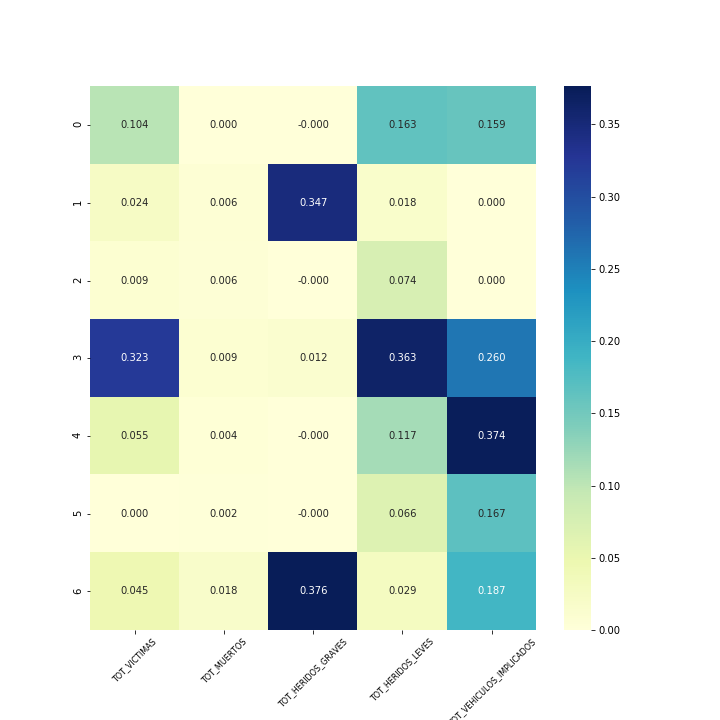
\includegraphics[width=0.9\textwidth]{imagenes/case2/kmeans/heatmaps/hm_kmeans_case2_entrada_k7.png}
\end{subfigure}
\caption{Mapas de calor para el algoritmo K-Means, P.M}
\label{fig:hm-km}
\end{figure}

\begin{figure}[H]
\begin{subfigure}{.5\textwidth}
  \centering
  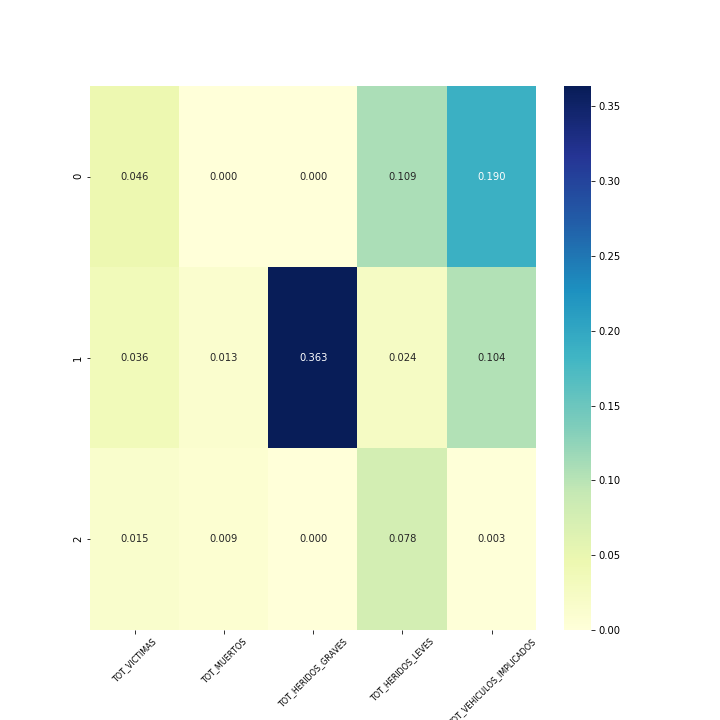
\includegraphics[width=0.9\textwidth]{imagenes/case2/agglomerative/heatmaps/hm_agglomerative_case2_entrada_k3.png}
\end{subfigure}%
\begin{subfigure}{.5\textwidth}
  \centering
  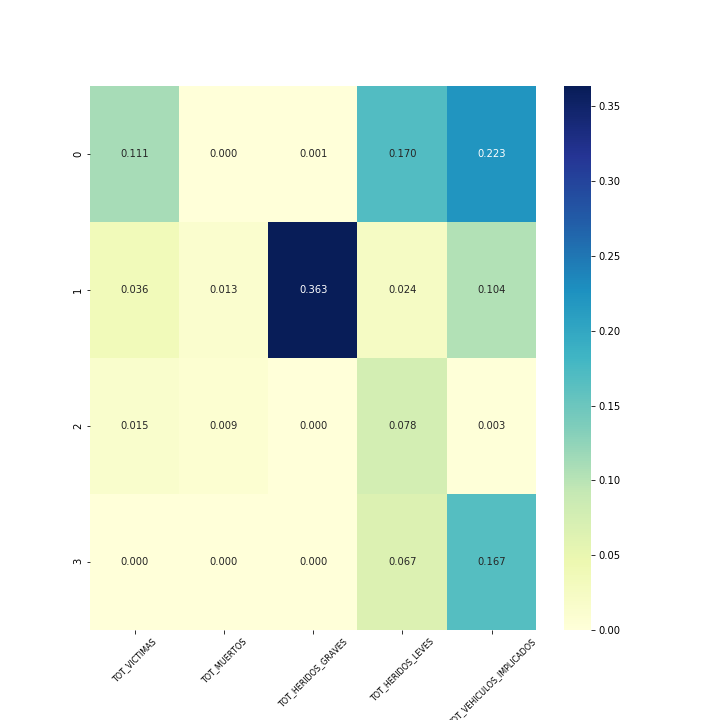
\includegraphics[width=0.9\textwidth]{imagenes/case2/agglomerative/heatmaps/hm_agglomerative_case2_entrada_k4.png}
\end{subfigure}
\begin{subfigure}{.5\textwidth}
  \centering
  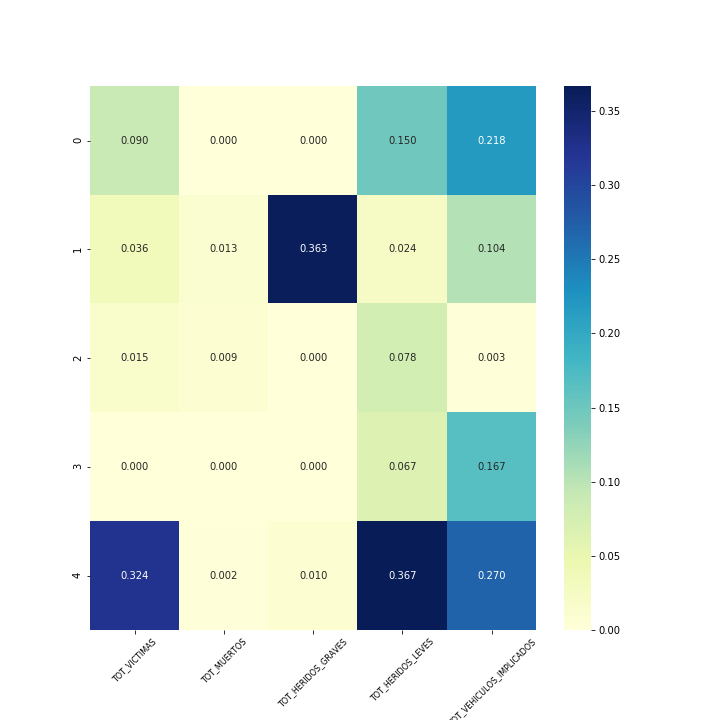
\includegraphics[width=0.9\textwidth]{imagenes/case2/agglomerative/heatmaps/hm_agglomerative_case2_entrada_k5.png}
\end{subfigure}
\begin{subfigure}{.5\textwidth}
  \centering
  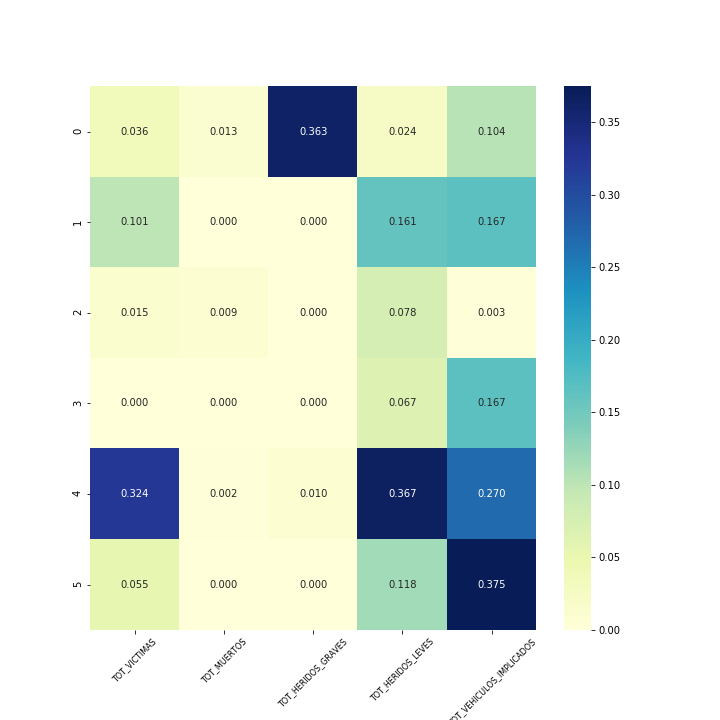
\includegraphics[width=0.9\textwidth]{imagenes/case2/agglomerative/heatmaps/hm_agglomerative_case2_entrada_k6.png}
\end{subfigure}
\begin{subfigure}{.5\textwidth}
  \centering
  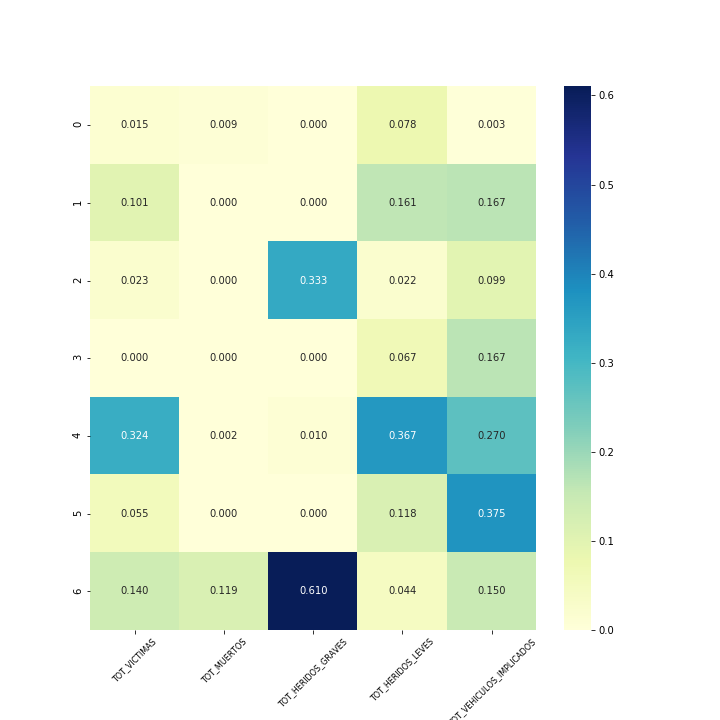
\includegraphics[width=0.9\textwidth]{imagenes/case2/agglomerative/heatmaps/hm_agglomerative_case2_entrada_k7.png}
\end{subfigure}
\caption{Mapas de calor para el algoritmo Agglomerative Clustering, P.M}
\label{fig:hm-km}
\end{figure}

\begin{figure}[H]
\begin{subfigure}{.5\textwidth}
  \centering
  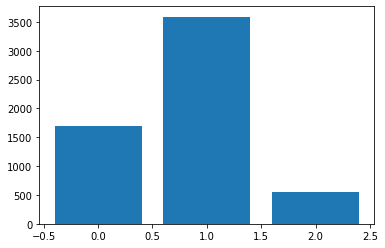
\includegraphics[width=0.45\textwidth]{imagenes/counter/pm/km3.png}
  \caption{$k=3$}
\end{subfigure}%
\begin{subfigure}{.5\textwidth}
  \centering
  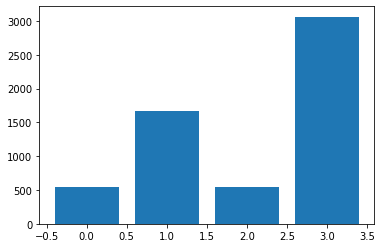
\includegraphics[width=0.45\textwidth]{imagenes/counter/pm/km4.png}
  \caption{$k=4$}
\end{subfigure}
\begin{subfigure}{.5\textwidth}
  \centering
  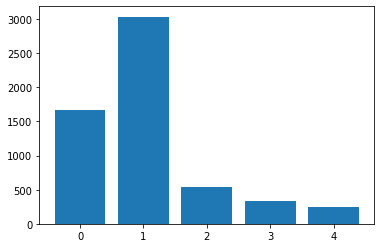
\includegraphics[width=0.45\textwidth]{imagenes/counter/pm/km5.png}
  \caption{$k=5$}
\end{subfigure}
\begin{subfigure}{.5\textwidth}
  \centering
  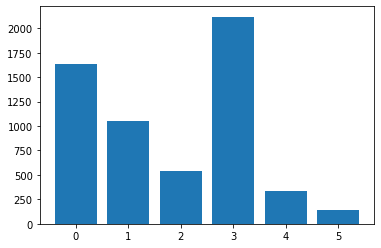
\includegraphics[width=0.45\textwidth]{imagenes/counter/pm/km6.png}
  \caption{$k=6$}
\end{subfigure}
\begin{subfigure}{.5\textwidth}
  \centering
  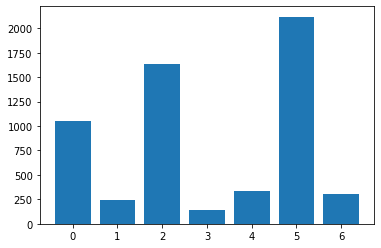
\includegraphics[width=0.45\textwidth]{imagenes/counter/pm/km7.png}
  \caption{$k=7$}
\end{subfigure}
\caption{Número de instancias en cada cluster(K-Means), P.M}
\label{fig:hm-km}
\end{figure}


\begin{figure}[H]
\begin{subfigure}{.5\textwidth}
  \centering
  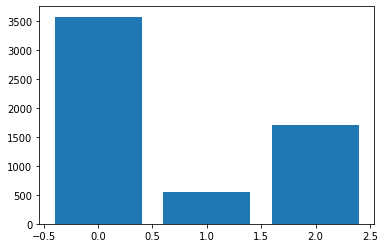
\includegraphics[width=0.45\textwidth]{imagenes/counter/pm/agg3.png}
  \caption{$k=3$}
\end{subfigure}%
\begin{subfigure}{.5\textwidth}
  \centering
  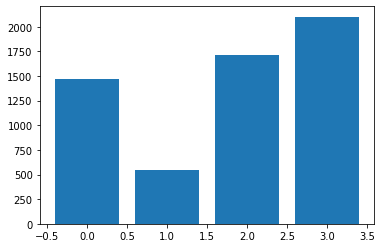
\includegraphics[width=0.45\textwidth]{imagenes/counter/pm/agg4.png}
  \caption{$k=4$}
\end{subfigure}
\begin{subfigure}{.5\textwidth}
  \centering
  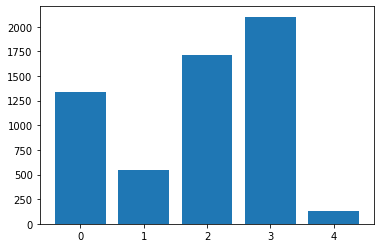
\includegraphics[width=0.45\textwidth]{imagenes/counter/pm/agg5.png}
  \caption{$k=5$}
\end{subfigure}
\begin{subfigure}{.5\textwidth}
  \centering
  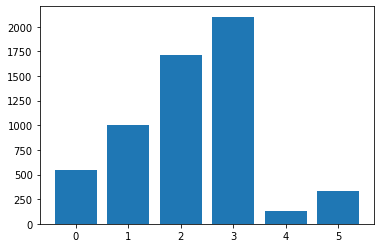
\includegraphics[width=0.45\textwidth]{imagenes/counter/pm/agg6.png}
  \caption{$k=6$}
\end{subfigure}
\begin{subfigure}{.5\textwidth}
  \centering
  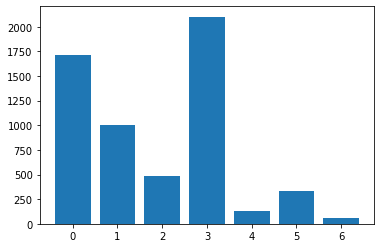
\includegraphics[width=0.45\textwidth]{imagenes/counter/pm/agg7.png}
  \caption{$k=7$}
\end{subfigure}
\caption{Número de instancias en cada cluster(Agglomerative-Clustering), P.M}
\label{fig:hm-km}
\end{figure}

En los agrupamientos se puede ver como separa bien, en unos teniendo apenas heridos y un vehículo implicado, serán atropellos. Y como dependiendo del número de heridos leves y vehiculos implicados va segmentando las instancias.

En comparación con el tramo de la madrugada, aquí aparecen cifras de muertos mayor que cero en más de un cluster, cuando en el caso opuesto se agrupan todas en uno(parece ser colisión con obstáculo o salida de vía). Además de mayores cifras en heridos leves y victimas en distintos clusters con respecto a la madrugada.

